\begin{figure}[t]
\centering
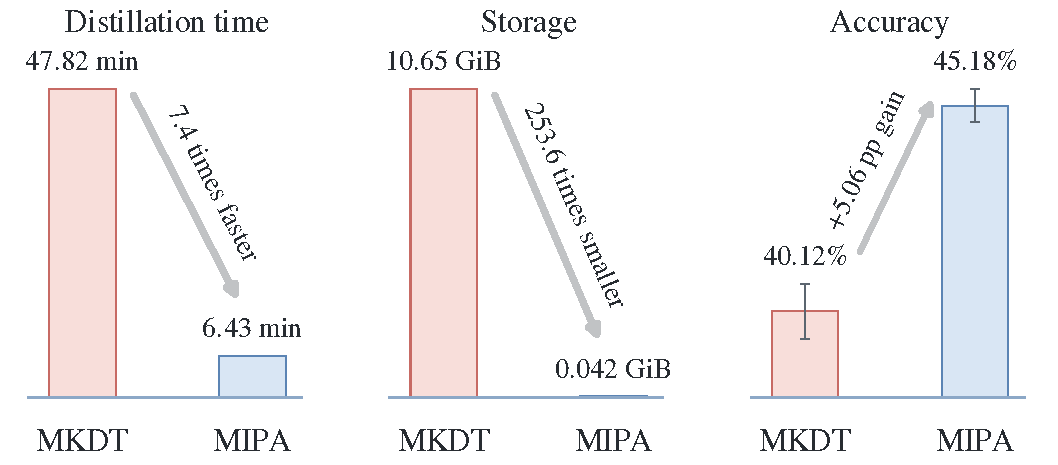
\includegraphics[width=\linewidth]{intro_figs/mipa_mkdt_cifar10_p0p2_lbl1/comparison.pdf}
\caption{\textbf{MIPA versus MKDT on CIFAR-10.} Both use 100 synthetic images (0.2\% data), followed by 2k-epoch SimCLR with ResNet-18 and a 1\%-label linear probe. Left: observed optimization time per update on one L40S, excluding initialization and teacher/expert preparation. MKDT uses 5k updates (47.82 min total); MIPA uses 10k (6.08 min). Right: mean accuracy with sample SD; MKDT pools six probes from two SSL seeds, and MIPA uses five probes from one SSL seed. Timings are historical observations from different nodes and dates.}
\label{fig:mipa-mkdt-cifar10-efficiency}
\end{figure}
